\begin{task}
\TT{Wyznacz współczynniki zespolonego szeregu Fouriera dla okresowego sygnału $f(t)$ przedstawionego na rysunku. Narysuj widmo amplitudowe i fazowe sygnału.}{Calculate coefficients of the periodic signal $f(t)$ shown below for the expansion into a complex exponential Fourier series. Draw magnitude and phase spectra.}

\begin{figure}[H]
\centering
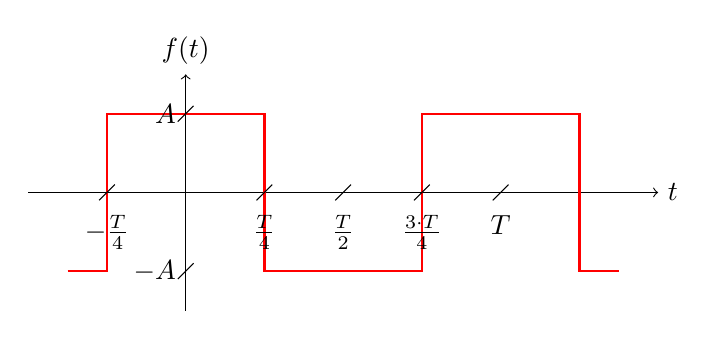
\begin{tikzpicture}
  %\draw (0,0) circle (1in);
  \draw[->] (-2.0,+0.0) -- (+6.0,+0.0) node[right] {$t$};
  \draw[->] (+0.0,-1.5) -- (+0.0,+1.5) node[above] {$f(t)$};
  \draw[-,red, thick] (-1.5,-1.0) -- (-1.0,-1.0) -- (-1.0,+1.0) -- (+1.0,+1.0) -- (+1.0,-1.0)--(+3.0,-1.0) -- (+3.0,+1.0) -- (+5.0,+1.0) -- (+5.0,-1.0) -- (+5.5,-1.0);
  %\draw[-] (-1.0-0.1,-0.1)--(-1.0+0.1,0.1) node[midway, below, outer sep=10pt,align=center] {$-\frac{T}{2}$};
  \draw[-] (-1.0-0.1,-0.1)--(-1.0+0.1,0.1) node[midway, below, outer sep=5pt,align=center] {$-\frac{T}{4}$};
  \draw[-] (+1.0-0.1,-0.1)--(+1.0+0.1,0.1) node[midway, below, outer sep=5pt] {$\frac{T}{4}$};
  \draw[-] (+2.0-0.1,-0.1)--(+2.0+0.1,0.1) node[midway, below, outer sep=5pt] {$\frac{T}{2}$};
  \draw[-] (+3.0-0.1,-0.1)--(+3.0+0.1,0.1) node[midway, below, outer sep=5pt] {$\frac{3\cdot T}{4}$};
  \draw[-] (+4.0-0.1,-0.1)--(+4.0+0.1,0.1) node[midway, below, outer sep=5pt] {$T$};
  \draw[-] (-0.1,+1.0-0.1)--(+0.1,+1.0+0.1) node[midway, left] {$A$};
  \draw[-] (-0.1,-1.0-0.1)--(+0.1,-1.0+0.1) node[midway, left] {$-A$};
\end{tikzpicture}
\end{figure}

\TT{W pierwszej kolejności należy opisać sygnał za pomocą wzoru.}{Periodic signal $f(t)$, as a piecewise linear function assuming period $t \in \left(\frac{-T}{4};\frac{3 \cdot T}{4}\right)$ is given by:}

\begin{equation}
    f(x)=\begin{cases}A & t \in \left (  -\frac{T}{4}+k \cdot T; \frac{T}{4}+k \cdot T \right ) \\
    -A & t \in \left (  \frac{T}{4}+k \cdot T; \frac{3\cdot T}{4} +k \cdot T\right )\end{cases} \wedge k \in \TT{C}{Z}
\end{equation}

\TT{Współczynnik $F_0$ wyznaczamy ze wzoru:}{The $F_0$ coefficient is defined as:}

\begin{equation}
F_0=\frac{1}{T}\int_{T}f(t) \cdot dt
\end{equation}

\TT{Podstawiamy do wzoru wzór naszej funkcji w pierwszym okresie $k=0$}{For the period $t \in (-\frac{T}{4}; \frac{3\cdot T}{4})$, i.e. $k=0$, we get:}

\begin{equation}
\begin{aligned}
F_0 &=\frac{1}{T}\int_{T}f(t) \cdot dt =\\
&=\frac{1}{T} \left( \int_{-\frac{T}{4}}^{\frac{T}{4}} A \cdot dt + \int_{\frac{T}{4}}^{\frac{3\cdot T}{4}} (-A) \cdot dt \right ) = \\
&=\frac{1}{T} \left( A \cdot \int_{-\frac{T}{4}}^{\frac{T}{4}} dt - A \cdot  \int_{\frac{T}{4}}^{\frac{3\cdot T}{4}} dt \right ) = \\
&=\frac{A}{T} \left( \left. t\right |_{-\frac{T}{4}}^{\frac{T}{4}} -\left. t\right |_{\frac{T}{4}}^{\frac{3 \cdot T}{4}} \right ) = \\
&=\frac{A}{T} \cdot \left[\left( \frac{T}{4} - \left(-\frac{T}{4}\right) \right ) - \left( \frac{3 \cdot T}{4} - \frac{T}{4} \right ) \right]= \\
&=\frac{A}{T} \cdot \left[ \frac{T}{4} + \frac{T}{4} - \frac{3 \cdot T}{4} + \frac{T}{4} \right]= \\
&=\frac{A}{T} \cdot \left[0 \right]= \\
&=0
\end{aligned}
\end{equation}

\TT{Wartość współczynnika $F_0$ wynosi $0$.}{The $F_0$ coefficient equals $0$.}


\TT{Współczynniki $F_k$ wyznaczamy ze wzoru:}{The $F_k$ coefficients are defined as:}


\begin{equation}
F_k=\frac{1}{T}\int_{T}f(t) \cdot e^{- \jmath \cdot k \cdot \frac{2\pi}{T} \cdot t} \cdot dt
\end{equation}

\TT{Podstawiamy do wzoru wzór naszej funkcji w pierwszym okresie $k=0$}{For the period $t \in (-\frac{T}{4}; \frac{3\cdot T}{4})$, i.e. $k=0$, we get:}

\begin{align*}
F_k&=\frac{1}{T}\int_{T}f(t) \cdot e^{-\jmath \cdot k \cdot \frac{2\pi}{T} \cdot t} \cdot dt=\\
&=\frac{1}{T} \left( \int_{-\frac{T}{4}}^{\frac{T}{4}} A \cdot e^{-\jmath \cdot k \cdot \frac{2\pi}{T} \cdot t} \cdot dt + \int_{\frac{T}{4}}^{\frac{3\cdot T}{4}} (-A) \cdot e^{-\jmath \cdot k \cdot \frac{2\pi}{T} \cdot t} \cdot dt \right ) = \\
&=\frac{1}{T} \left( A \cdot \int_{-\frac{T}{4}}^{\frac{T}{4}} e^{-\jmath \cdot k \cdot \frac{2\pi}{T} \cdot t} \cdot dt - A \cdot  \int_{\frac{T}{4}}^{\frac{3\cdot T}{4}} e^{-\jmath \cdot k \cdot \frac{2\pi}{T} \cdot t} \cdot dt \right ) = \\
&=\frac{A}{T} \left( \int_{-\frac{T}{4}}^{\frac{T}{4}} e^{-\jmath \cdot k \cdot \frac{2\pi}{T} \cdot t} \cdot dt - \int_{\frac{T}{4}}^{\frac{3\cdot T}{4}} e^{-\jmath \cdot k \cdot \frac{2\pi}{T} \cdot t} \cdot dt \right ) = \\
&=\begin{Bmatrix*}[l]
z&=-\jmath \cdot k\cdot \frac{2\pi}{T} \cdot t\\
dz&=-\jmath \cdot k\cdot \frac{2\pi}{T} \cdot dt\\
dt&=\frac{dz}{-\jmath \cdot k\cdot \frac{2\pi}{T}}
\end{Bmatrix*}=\\
&=\frac{A}{T} \left[ \int_{-\frac{T}{4}}^{\frac{T}{4}} e^{z} \cdot \frac{dz}{-\jmath \cdot k\cdot \frac{2\pi}{T}} -\int_{\frac{T}{4}}^{\frac{3\cdot T}{4}} e^{z} \cdot \frac{dz}{-\jmath \cdot k\cdot \frac{2\pi}{T}} \right]=\\
&=\frac{-A}{T \cdot \jmath \cdot k\cdot \frac{2\pi}{T}} \left[  \int_{-\frac{T}{4}}^{\frac{T}{4}} e^{z} \cdot dz - \int_{\frac{T}{4}}^{\frac{3\cdot T}{4}} e^{z} \cdot dz \right]=\\
&=\frac{-A}{\jmath \cdot k\cdot 2 \pi} \left[ \left. e^{z} \right|_{-\frac{T}{4}}^{\frac{T}{4}} - \left. e^{z} \right|_{\frac{T}{4}}^{\frac{3 \cdot T}{4}}\right]=\\
&=\frac{-A}{\jmath \cdot k\cdot 2 \pi} \left[ \left. e^{-\jmath \cdot k\cdot \frac{2\pi}{T} \cdot t} \right|_{-\frac{T}{4}}^{\frac{T}{4}} - \left. e^{-\jmath \cdot k\cdot \frac{2\pi}{T} \cdot t} \right|_{\frac{T}{4}}^{\frac{3 \cdot T}{4}}\right]=\\
&=\frac{-A}{\jmath \cdot k\cdot 2 \pi}\left( e^{-\jmath \cdot k\cdot \frac{2\pi}{T} \cdot \frac{T}{4}} - e^{-\jmath \cdot k\cdot \frac{2\pi}{T} \cdot \left(-\frac{T}{4}\right)} - e^{-\jmath \cdot k\cdot \frac{2\pi}{T} \cdot \frac{3 \cdot T}{4}} + e^{-\jmath \cdot k\cdot \frac{2\pi}{T} \cdot \frac{T}{4}}\right)=\\
&=\frac{-A}{\jmath \cdot k\cdot 2 \pi}\left( e^{-\jmath \cdot k\cdot \frac{\pi}{2}} - e^{\jmath \cdot k\cdot \frac{\pi}{2}} - e^{-\jmath \cdot k\cdot \frac{3\pi}{2}} + e^{-\jmath \cdot k\cdot \frac{\pi}{2}}\right)=\\
&=\begin{Bmatrix*}[l]
e^{-\jmath \cdot k\cdot \frac{3\pi}{2}} = e^{-\jmath \cdot k\cdot \left(2\pi - \frac{\pi}{2}\right)} = e^{-\jmath \cdot k\cdot 2\pi} \cdot  e^{\jmath \cdot k\cdot \frac{\pi}{2}} = 1 \cdot  e^{\jmath \cdot k\cdot \frac{\pi}{2}} = e^{\jmath \cdot k\cdot \frac{\pi}{2}}
\end{Bmatrix*}=\\
&=\frac{-A}{\jmath \cdot k\cdot 2 \pi}\left( e^{-\jmath \cdot k\cdot \frac{\pi}{2}} - e^{\jmath \cdot k\cdot \frac{\pi}{2}} - e^{\jmath \cdot k\cdot \frac{\pi}{2}} + e^{-\jmath \cdot k\cdot \frac{\pi}{2}}\right)=\\
&=\frac{-A}{\jmath \cdot k\cdot 2 \pi}\left( 2 \cdot e^{-\jmath \cdot k\cdot \frac{\pi}{2}} - 2 \cdot e^{\jmath \cdot k\cdot \frac{\pi}{2}}\right)=\\
&=\frac{2 \cdot A}{\jmath \cdot k\cdot 2 \pi}\left( e^{\jmath \cdot k\cdot \frac{\pi}{2}} - e^{-\jmath \cdot k\cdot \frac{\pi}{2}}\right)=\\
&=\frac{2 \cdot A}{k\cdot \pi}\left( sin \left(k\cdot \frac{\pi}{2}\right)\right)
\end{align*}

\TT{Wartość współczynnika $F_k$ wynosi $\frac{2 \cdot A}{k\cdot \pi}\left( sin \left(k\cdot \frac{\pi}{2}\right)\right)$.}{The $F_k$ coefficients equal to $\frac{2 \cdot A}{k\cdot \pi}\left( sin \left(k\cdot \frac{\pi}{2}\right)\right)$.}


\TT{Ostatecznie współczynniki zespolonego szeregu Fouriera dla funkcji przedstawionej na rysunku przyjmują wartości:}{To sum up, coefficients for the expansion into a complex exponential Fourier series are given by:}

\begin{align*}
F_0&=0\\
F_k&=\frac{2 \cdot A}{k\cdot \pi}\left( sin \left(k\cdot \frac{\pi}{2}\right)\right)\\
\end{align*}

\TT{Możemy wyznaczyć kilka wartości współczynników $F_k$:}{The first several coefficients are equal to:}

\begin{table}[H]
    \centering  
    \begin{tabular}{|c|c|c|c|c|c|c|c|c|c|c|c|c|}
        \hline 
        $k$ & $-5$ & $-4$ & $-3$ & $-2$ & $-1$ & $0$ & $1$ & $2$ & $3$ & $4$ & $5$\\ 
        \hline 
        $F_k$ & $\frac{2\cdot A}{5 \cdot \pi}$ & $0$ & $-\frac{2\cdot A}{3 \cdot \pi}$ & $0$ & $\frac{2\cdot A}{\pi}$ & $0$ & $\frac{2\cdot A}{\pi}$ & $0$ & $-\frac{2 \cdot A}{3 \cdot \pi}$ & $0$ & $\frac{2\cdot A}{5 \cdot \pi}$\\ 
        \hline 
        $\left| F_k \right|$ & $\frac{2\cdot A}{5 \cdot \pi}$ & $0$ & $\frac{2\cdot A}{3 \cdot \pi}$ & $0$ & $\frac{2\cdot A}{\pi}$ & $0$ & $\frac{2\cdot A}{\pi}$ & $0$ & $\frac{2 \cdot A}{3 \cdot \pi}$ & $0$ & $\frac{2\cdot A}{5 \cdot \pi}$\\
        \hline
        $Arg\left\{ F_k \right\}$ & $0$ & $0$ & $-\pi$ & $0$ & $0$ & $0$ & $0$ & $0$ & $\pi$ & $0$ & $0$\\
        \hline
    \end{tabular} 
\end{table}

\TT{Podstawiając wyznaczone współczynniki do wzoru aproksymacyjnego, funkcję $f(t)$ możemy wyrazić jako:}{Hence, the signal $f(t)$ may be expressed as the sum of the harmonic series}

\begin{equation}
\begin{aligned}
f(t) &= \sum_{k=-\infty}^{\infty} F_k \cdot e^{\jmath \cdot k \cdot \frac{2\pi}{T} \cdot t}\\
f(t) &= \sum_{\begin{smallmatrix}k=-\infty \\ k \neq 0 \end{smallmatrix}}^{\infty} \left[\frac{2 \cdot A}{k\cdot \pi}\left( sin \left(k \cdot \frac{\pi}{2}\right)\right)\right] \cdot e^{\jmath \cdot k \cdot \frac{2\pi}{T} \cdot t}\\
\end{aligned}
\end{equation}

\TT{W przypadku sumowania od $k_{min}=-1$ do $k_{max}=1$ otrzymujemy:}{A partial approximation of the $f(t)$ signal from $k_{min}=-1$ to $k_{max}=1$ results in:}

\begin{figure}[H]
  \centering
  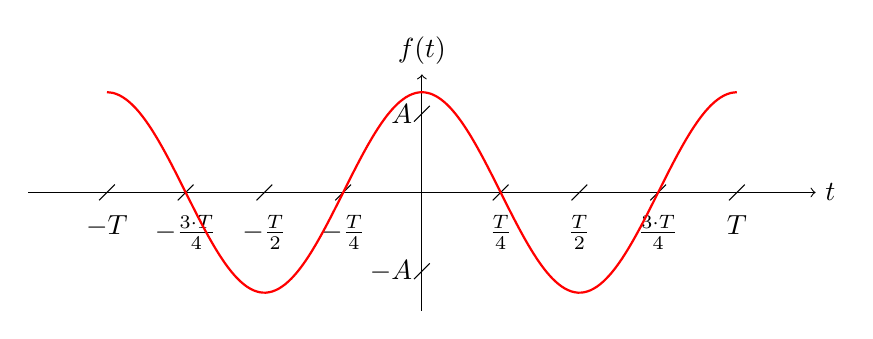
\begin{tikzpicture}
  \draw[->] (-5.0,+0.0) -- (+5.0,+0.0) node[right] {$t$};
  \draw[->] (+0.0,-1.5) -- (+0.0,+1.5) node[above] {$f(t)$};
  \draw[-] (-4.0-0.1,-0.1)--(-4.0+0.1,0.1) node[midway, below, outer sep=5pt] {$-T$};
  \draw[-] (-3.0-0.1,-0.1)--(-3.0+0.1,0.1) node[midway, below, outer sep=5pt] {$-\frac{3\cdot T}{4}$};
  \draw[-] (-2.0-0.1,-0.1)--(-2.0+0.1,0.1) node[midway, below, outer sep=5pt,align=center] {$-\frac{T}{2}$};
  \draw[-] (-1.0-0.1,-0.1)--(-1.0+0.1,0.1) node[midway, below, outer sep=5pt,align=center] {$-\frac{T}{4}$};
  \draw[-] (+1.0-0.1,-0.1)--(+1.0+0.1,0.1) node[midway, below, outer sep=5pt] {$\frac{T}{4}$};
  \draw[-] (+2.0-0.1,-0.1)--(+2.0+0.1,0.1) node[midway, below, outer sep=5pt] {$\frac{T}{2}$};
  \draw[-] (+3.0-0.1,-0.1)--(+3.0+0.1,0.1) node[midway, below, outer sep=5pt] {$\frac{3\cdot T}{4}$};
  \draw[-] (+4.0-0.1,-0.1)--(+4.0+0.1,0.1) node[midway, below, outer sep=5pt] {$T$};
  \draw[-] (-0.1,1.0-0.1)--(+0.1,1.0+0.1) node[midway, left] {$A$};
  \draw[-] (-0.1,-1.0-0.1)--(+0.1,-1.0+0.1) node[midway, left] {$-A$};
  
  \draw[scale=1.0,domain=-4:4.0,samples=100,smooth,variable=\x,red,thick] plot ({\x},{4.0/3.141592*cos(\x*180.0/2)});
  \end{tikzpicture}
\end{figure}

\TT{W przypadku sumowania od $k_{min}=-3$ do $k_{max}=3$ otrzymujemy:}{A partial approximation of the $f(t)$ signal from $k_{min}=-3$ to $k_{max}=3$ results in:}

\begin{figure}[H]
    \centering
    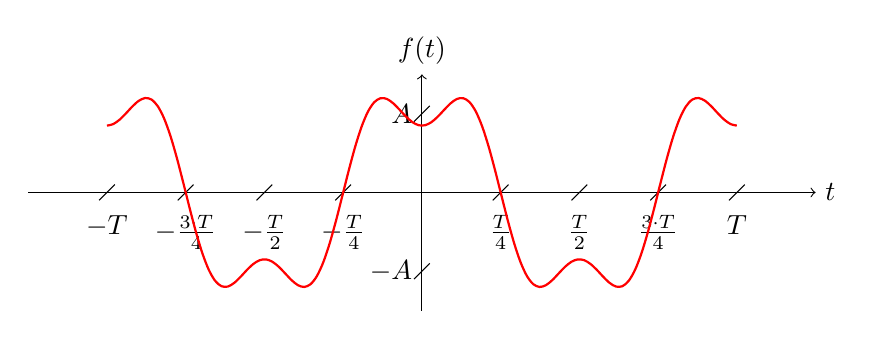
\begin{tikzpicture}
    \draw[->] (-5.0,+0.0) -- (+5.0,+0.0) node[right] {$t$};
    \draw[->] (+0.0,-1.5) -- (+0.0,+1.5) node[above] {$f(t)$};
    \draw[-] (-4.0-0.1,-0.1)--(-4.0+0.1,0.1) node[midway, below, outer sep=5pt] {$-T$};
    \draw[-] (-3.0-0.1,-0.1)--(-3.0+0.1,0.1) node[midway, below, outer sep=5pt] {$-\frac{3\cdot T}{4}$};
    \draw[-] (-2.0-0.1,-0.1)--(-2.0+0.1,0.1) node[midway, below, outer sep=5pt,align=center] {$-\frac{T}{2}$};
    \draw[-] (-1.0-0.1,-0.1)--(-1.0+0.1,0.1) node[midway, below, outer sep=5pt,align=center] {$-\frac{T}{4}$};
    \draw[-] (+1.0-0.1,-0.1)--(+1.0+0.1,0.1) node[midway, below, outer sep=5pt] {$\frac{T}{4}$};
    \draw[-] (+2.0-0.1,-0.1)--(+2.0+0.1,0.1) node[midway, below, outer sep=5pt] {$\frac{T}{2}$};
    \draw[-] (+3.0-0.1,-0.1)--(+3.0+0.1,0.1) node[midway, below, outer sep=5pt] {$\frac{3\cdot T}{4}$};
    \draw[-] (+4.0-0.1,-0.1)--(+4.0+0.1,0.1) node[midway, below, outer sep=5pt] {$T$};
    \draw[-] (-0.1,1.0-0.1)--(+0.1,1.0+0.1) node[midway, left] {$A$};
    \draw[-] (-0.1,-1.0-0.1)--(+0.1,-1.0+0.1) node[midway, left] {$-A$};
    
    \draw[scale=1.0,domain=-4:4.0,samples=100,smooth,variable=\x,red,thick] plot ({\x},{4.0/3.141592*cos(\x*180.0/2) - 4.0/(3*3.141592)*cos(\x*180.0/2*3)});
    \end{tikzpicture}
\end{figure}

\TT{W przypadku sumowania od $k_{min}=-5$ do $k_{max}=5$ otrzymujemy:}{A partial approximation of the $f(t)$ signal from $k_{min}=-5$ to $k_{max}=5$ results in:}

\begin{figure}[H]
    \centering
    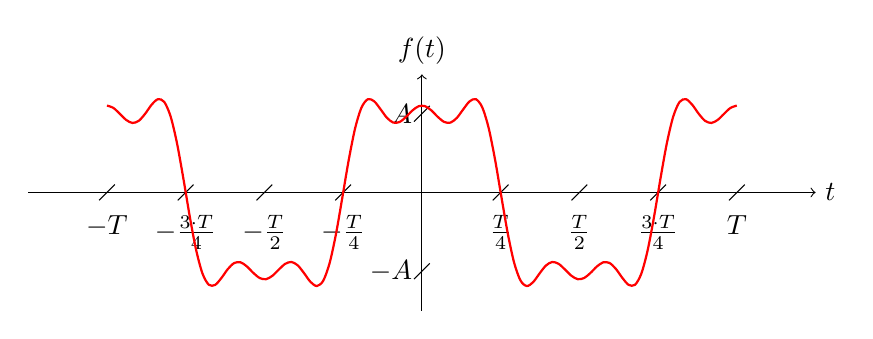
\begin{tikzpicture}
    \draw[->] (-5.0,+0.0) -- (+5.0,+0.0) node[right] {$t$};
    \draw[->] (+0.0,-1.5) -- (+0.0,+1.5) node[above] {$f(t)$};
    \draw[-] (-4.0-0.1,-0.1)--(-4.0+0.1,0.1) node[midway, below, outer sep=5pt] {$-T$};
    \draw[-] (-3.0-0.1,-0.1)--(-3.0+0.1,0.1) node[midway, below, outer sep=5pt] {$-\frac{3\cdot T}{4}$};
    \draw[-] (-2.0-0.1,-0.1)--(-2.0+0.1,0.1) node[midway, below, outer sep=5pt,align=center] {$-\frac{T}{2}$};
    \draw[-] (-1.0-0.1,-0.1)--(-1.0+0.1,0.1) node[midway, below, outer sep=5pt,align=center] {$-\frac{T}{4}$};
    \draw[-] (+1.0-0.1,-0.1)--(+1.0+0.1,0.1) node[midway, below, outer sep=5pt] {$\frac{T}{4}$};
    \draw[-] (+2.0-0.1,-0.1)--(+2.0+0.1,0.1) node[midway, below, outer sep=5pt] {$\frac{T}{2}$};
    \draw[-] (+3.0-0.1,-0.1)--(+3.0+0.1,0.1) node[midway, below, outer sep=5pt] {$\frac{3\cdot T}{4}$};
    \draw[-] (+4.0-0.1,-0.1)--(+4.0+0.1,0.1) node[midway, below, outer sep=5pt] {$T$};
    \draw[-] (-0.1,1.0-0.1)--(+0.1,1.0+0.1) node[midway, left] {$A$};
    \draw[-] (-0.1,-1.0-0.1)--(+0.1,-1.0+0.1) node[midway, left] {$-A$};
    
    \draw[scale=1.0,domain=-4:4.0,samples=100,smooth,variable=\x,red,thick] plot ({\x},{4.0/3.141592*cos(\x*180.0/2) - 4.0/(3*3.141592)*cos(\x*180.0/2*3) + 4.0/(5*3.141592)*cos(\x*180.0/2*5)});
    \end{tikzpicture}
\end{figure}

\TT{W przypadku sumowania od $k_{min}=-11$ do $k_{max}=11$ otrzymujemy:}{A partial approximation of the $f(t)$ signal from $k_{min}=-11$ to $k_{max}=11$ results in:}

\begin{figure}[H]
    \centering
    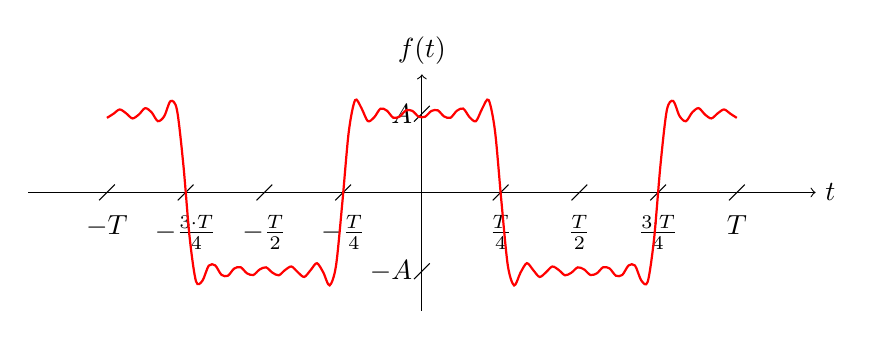
\begin{tikzpicture}
    \draw[->] (-5.0,+0.0) -- (+5.0,+0.0) node[right] {$t$};
    \draw[->] (+0.0,-1.5) -- (+0.0,+1.5) node[above] {$f(t)$};
    \draw[-] (-4.0-0.1,-0.1)--(-4.0+0.1,0.1) node[midway, below, outer sep=5pt] {$-T$};
    \draw[-] (-3.0-0.1,-0.1)--(-3.0+0.1,0.1) node[midway, below, outer sep=5pt] {$-\frac{3\cdot T}{4}$};
    \draw[-] (-2.0-0.1,-0.1)--(-2.0+0.1,0.1) node[midway, below, outer sep=5pt,align=center] {$-\frac{T}{2}$};
    \draw[-] (-1.0-0.1,-0.1)--(-1.0+0.1,0.1) node[midway, below, outer sep=5pt,align=center] {$-\frac{T}{4}$};
    \draw[-] (+1.0-0.1,-0.1)--(+1.0+0.1,0.1) node[midway, below, outer sep=5pt] {$\frac{T}{4}$};
    \draw[-] (+2.0-0.1,-0.1)--(+2.0+0.1,0.1) node[midway, below, outer sep=5pt] {$\frac{T}{2}$};
    \draw[-] (+3.0-0.1,-0.1)--(+3.0+0.1,0.1) node[midway, below, outer sep=5pt] {$\frac{3\cdot T}{4}$};
    \draw[-] (+4.0-0.1,-0.1)--(+4.0+0.1,0.1) node[midway, below, outer sep=5pt] {$T$};
    \draw[-] (-0.1,1.0-0.1)--(+0.1,1.0+0.1) node[midway, left] {$A$};
    \draw[-] (-0.1,-1.0-0.1)--(+0.1,-1.0+0.1) node[midway, left] {$-A$};
    
    \draw[scale=1.0,domain=-4:4.0,samples=100,smooth,variable=\x,red,thick] plot ({\x},{4.0/3.141592*cos(\x*180.0/2) - 4.0/(3*3.141592)*cos(\x*180.0/2*3) + 4.0/(5*3.141592)*cos(\x*180.0/2*5) - 4.0/(7*3.141592)*cos(\x*180.0/2*7) + 4.0/(9*3.141592)*cos(\x*180.0/2*9)- 4.0/(11*3.141592)*cos(\x*180.0/2*11)});
    \end{tikzpicture}
\end{figure}

\TT{W przypadku sumowania od $k_{min}=-21$ do $k_{max}=21$ otrzymujemy:}{A partial approximation of the $f(t)$ signal from $k_{min}=-21$ to $k_{max}=21$ results in:}

\begin{figure}[H]
    \centering
    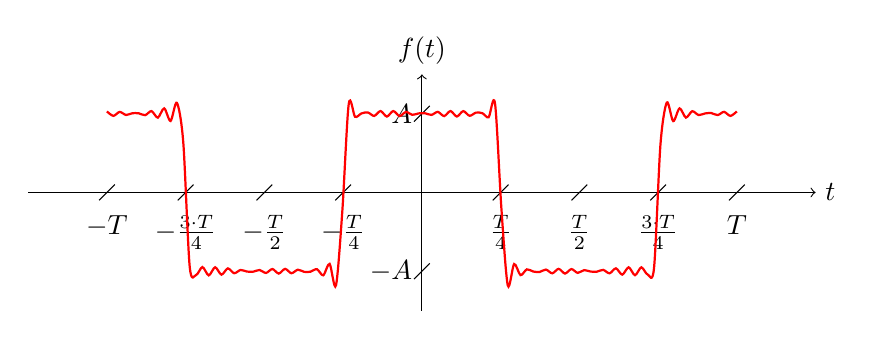
\begin{tikzpicture}
    \draw[->] (-5.0,+0.0) -- (+5.0,+0.0) node[right] {$t$};
    \draw[->] (+0.0,-1.5) -- (+0.0,+1.5) node[above] {$f(t)$};
    \draw[-] (-4.0-0.1,-0.1)--(-4.0+0.1,0.1) node[midway, below, outer sep=5pt] {$-T$};
    \draw[-] (-3.0-0.1,-0.1)--(-3.0+0.1,0.1) node[midway, below, outer sep=5pt] {$-\frac{3\cdot T}{4}$};
    \draw[-] (-2.0-0.1,-0.1)--(-2.0+0.1,0.1) node[midway, below, outer sep=5pt,align=center] {$-\frac{T}{2}$};
    \draw[-] (-1.0-0.1,-0.1)--(-1.0+0.1,0.1) node[midway, below, outer sep=5pt,align=center] {$-\frac{T}{4}$};
    \draw[-] (+1.0-0.1,-0.1)--(+1.0+0.1,0.1) node[midway, below, outer sep=5pt] {$\frac{T}{4}$};
    \draw[-] (+2.0-0.1,-0.1)--(+2.0+0.1,0.1) node[midway, below, outer sep=5pt] {$\frac{T}{2}$};
    \draw[-] (+3.0-0.1,-0.1)--(+3.0+0.1,0.1) node[midway, below, outer sep=5pt] {$\frac{3\cdot T}{4}$};
    \draw[-] (+4.0-0.1,-0.1)--(+4.0+0.1,0.1) node[midway, below, outer sep=5pt] {$T$};
    \draw[-] (-0.1,1.0-0.1)--(+0.1,1.0+0.1) node[midway, left] {$A$};
    \draw[-] (-0.1,-1.0-0.1)--(+0.1,-1.0+0.1) node[midway, left] {$-A$};
    
    \draw[scale=1.0,domain=-4:4.0,samples=100,smooth,variable=\x,red,thick] plot ({\x},{4.0/3.141592*cos(\x*180.0/2) - 4.0/(3*3.141592)*cos(\x*180.0/2*3) + 4.0/(5*3.141592)*cos(\x*180.0/2*5) - 4.0/(7*3.141592)*cos(\x*180.0/2*7) + 4.0/(9*3.141592)*cos(\x*180.0/2*9)- 4.0/(11*3.141592)*cos(\x*180.0/2*11) +
    4.0/(13*3.141592)*cos(\x*180.0/2*13) - 4.0/(15*3.141592)*cos(\x*180.0/2*15) + 4.0/(17*3.141592)*cos(\x*180.0/2*17) - 4.0/(19*3.141592)*cos(\x*180.0/2*19) + 4.0/(21*3.141592)*cos(\x*180.0/2*21)});
    \end{tikzpicture}
\end{figure}

\TT{W granicy sumowania od $k_{min}=-\infty$ do $k_{max}=\infty$ otrzymujemy oryginalny sygnał.}{Approximation of the $f(t)$ signal for from $k_{min}=-\infty$ to $k_{max}=\infty$ results in oryginal signal.}

\TT{Na podstawie wyznaczonych współczynników $F_k$ możemy narysować widmo amplitudowe $\left|F_k\right|$ sygnału $f(t)$.}{Based on coefficents $F_k$ we can plot magnitude spectrum $\left|F_k\right|$ of the $f(t)$ signal.}

\begin{figure}[H]
    \centering
    \begin{tikzpicture}
    
    \tikzmath{
        function mFk(\k,\A) {
            if(\k==0) then
            {
                return 0;
            }
            else
            {
                return abs(2* \A /(\k*3.141592)*(sin(\k*180/2));      
            };
        };
    }
    
    %\draw (0,0) circle (1in);
    \draw[->] (-6.0,+0.0) -- (+6.0,+0.0) node[right] {$k$};
    \draw[->] (+0.0,-0.0) -- (+0.0,+2.5) node[above] {$\left|F_k\right|$};
    \draw[-] (-0.1,2.0-0.1)--(+0.1,2.0+0.1) node[midway, left] {$\frac{2 \cdot A}{\pi}$};
    
    \foreach \k in {-8,-7,...,8 }{
        \pgfmathsetmacro{\x}{\k/1.5};
        \draw[-] ({\x-0.1},-0.1)--({\x+0.1},0.1) node[midway, below, outer sep=5pt] {${\k}$};    
    };
    
    \foreach \k in {-8,-7,...,8 }{
        \pgfmathsetmacro{\x}{\k/1.5};
        \pgfmathsetmacro{\y}{mFk(\k,4)*3.141592/4};
        \node[circle,red,fill=red,scale=0.5] (\x\y) at (\x,\y) {};
        \draw[-, red] (\x,0) -- (\x,\y);
    };
    
    \end{tikzpicture}
\end{figure}

\TT{Widmo aplitudowe sygnału rzeczywistego jest zawsze parzyste.}{The magnitude spectrum of a \underline{real signal} is an even-symmetric function of $k$.}

\TT{Podobnie n podstawie wyznaczonych współczynników $F_k$ możemy narysować widmo fazowe $\mathtt{arg}\left\{F_k\right\}$ sygnału $f(t)$.}{Based on coefficents $F_k$ we can plot phase spectrum $\mathtt{arg}\left\{F_k\right\}$ of the $f(t)$ signal.}

\begin{figure}[H]
    \centering
    \begin{tikzpicture}
    
    \tikzmath{
        function aFk(\k,\A) {
            if(\k==0) then
            {
                return 0;
            }
            else
            {
                if(mod(abs(\k),4))==3) then
                {
                    return 3.141592*sign(\k);
                }
                else
                {
                    return 0;                  
                };
            };
        };
    }
    
    %\draw (0,0) circle (1in);
    \draw[->] (-6.0,+0.0) -- (+6.0,+0.0) node[right] {$k$};
    \draw[->] (+0.0,-2.5) -- (+0.0,+2.5) node[above] {$\mathtt{arg}\left\{F_k\right\}$};
    \draw[-] (-0.1,2.0-0.1)--(+0.1,2.0+0.1) node[midway, left] {$\pi$};
    \draw[-] (-0.1,-2.0-0.1)--(+0.1,-2.0+0.1) node[midway, left] {$-\pi$};
    
    \foreach \k in {-8,-7,...,8 }{
        \pgfmathsetmacro{\x}{\k/1.5};
        \draw[-] ({\x-0.1},-0.1)--({\x+0.1},0.1) node[midway, below, outer sep=5pt] {${\k}$};    
    };
    
    \foreach \k in {-8,-7,...,8 }{
        \pgfmathsetmacro{\x}{\k/1.5};
        \pgfmathsetmacro{\y}{aFk(\k,4)*2.0/3.141592};
        \node[circle,red,fill=red,scale=0.5] (\x\y) at (\x,\y) {};
        \draw[-, red] (\x,0) -- (\x,\y);
    };
    
    \end{tikzpicture}
\end{figure}

\TT{Widmo fazowe sygnału rzeczywistego jest zawsze nieparzyste.}{The phase spectrum of a \underline{real signal} is an odd-symmetric function of $k$.}

\end{task}